\documentclass[a4paper, oneside]{memoir}
\usepackage[utf8]{inputenc}
\usepackage[T1]{fontenc}
\usepackage{pifont}
\usepackage{amssymb}
\usepackage{fourier}
\usepackage[dvipsnames]{xcolor}
\usepackage{tikz}
\usepackage{pdfpages}
\usepackage[sfdefault]{roboto}
\usepackage{color}

% Styles
\tikzstyle{teamshare} = [below, text width=5.4cm, inner sep = 0.5cm, text=white, align=center]
\tikzstyle{cardtext} = [below, text width=5.9cm, inner sep = 0.25cm, text centered]
\setlrmarginsandblock{0.9cm}{*}{1}
\setulmarginsandblock{1.49cm}{*}{1}
\checkandfixthelayout[nearest]
\pagestyle{empty}

% Define Commands
\newcommand{\condition}[1]{\textbf{#1}}
\newcommand{\character}[1]{\textbf{#1}}
\newdimen\titlespacing
\titlespacing=0.15cm

% Define Seperators
\newcommand{\seperator}[1]{\\ \vspace{\titlespacing} \hrulefill {} \tiny \bfseries #1 \normalfont \normalsize \hrulefill \\ \vspace{\titlespacing}}
\newcommand{\seperatoraction}{\seperator{POWER}}
\newcommand{\seperatordescription}{\seperator{DESCRIPTION}}
\newcommand{\seperatorcondition}{\seperator{CONDITION}}
\newcommand{\seperatorwin}{\seperator{HOW TO WIN}}
\newcommand{\redwinsection}{
	\seperatorwin
	\small You win if \character{President} gains the \condition{dead} condition due to the \character{Bomber} exploading.
}
\newcommand{\bluewinsection}{
	\seperatorwin
	\small You win if \character{President} does not gain the \condition{dead} condition due to the \character{Bomber} exploading.
}
\newcommand{\titlefrom}[1]{\\ \tiny > from #1 <\normalsize}

% Begin Document
\begin{document}
	
	% New Page
	\noindent 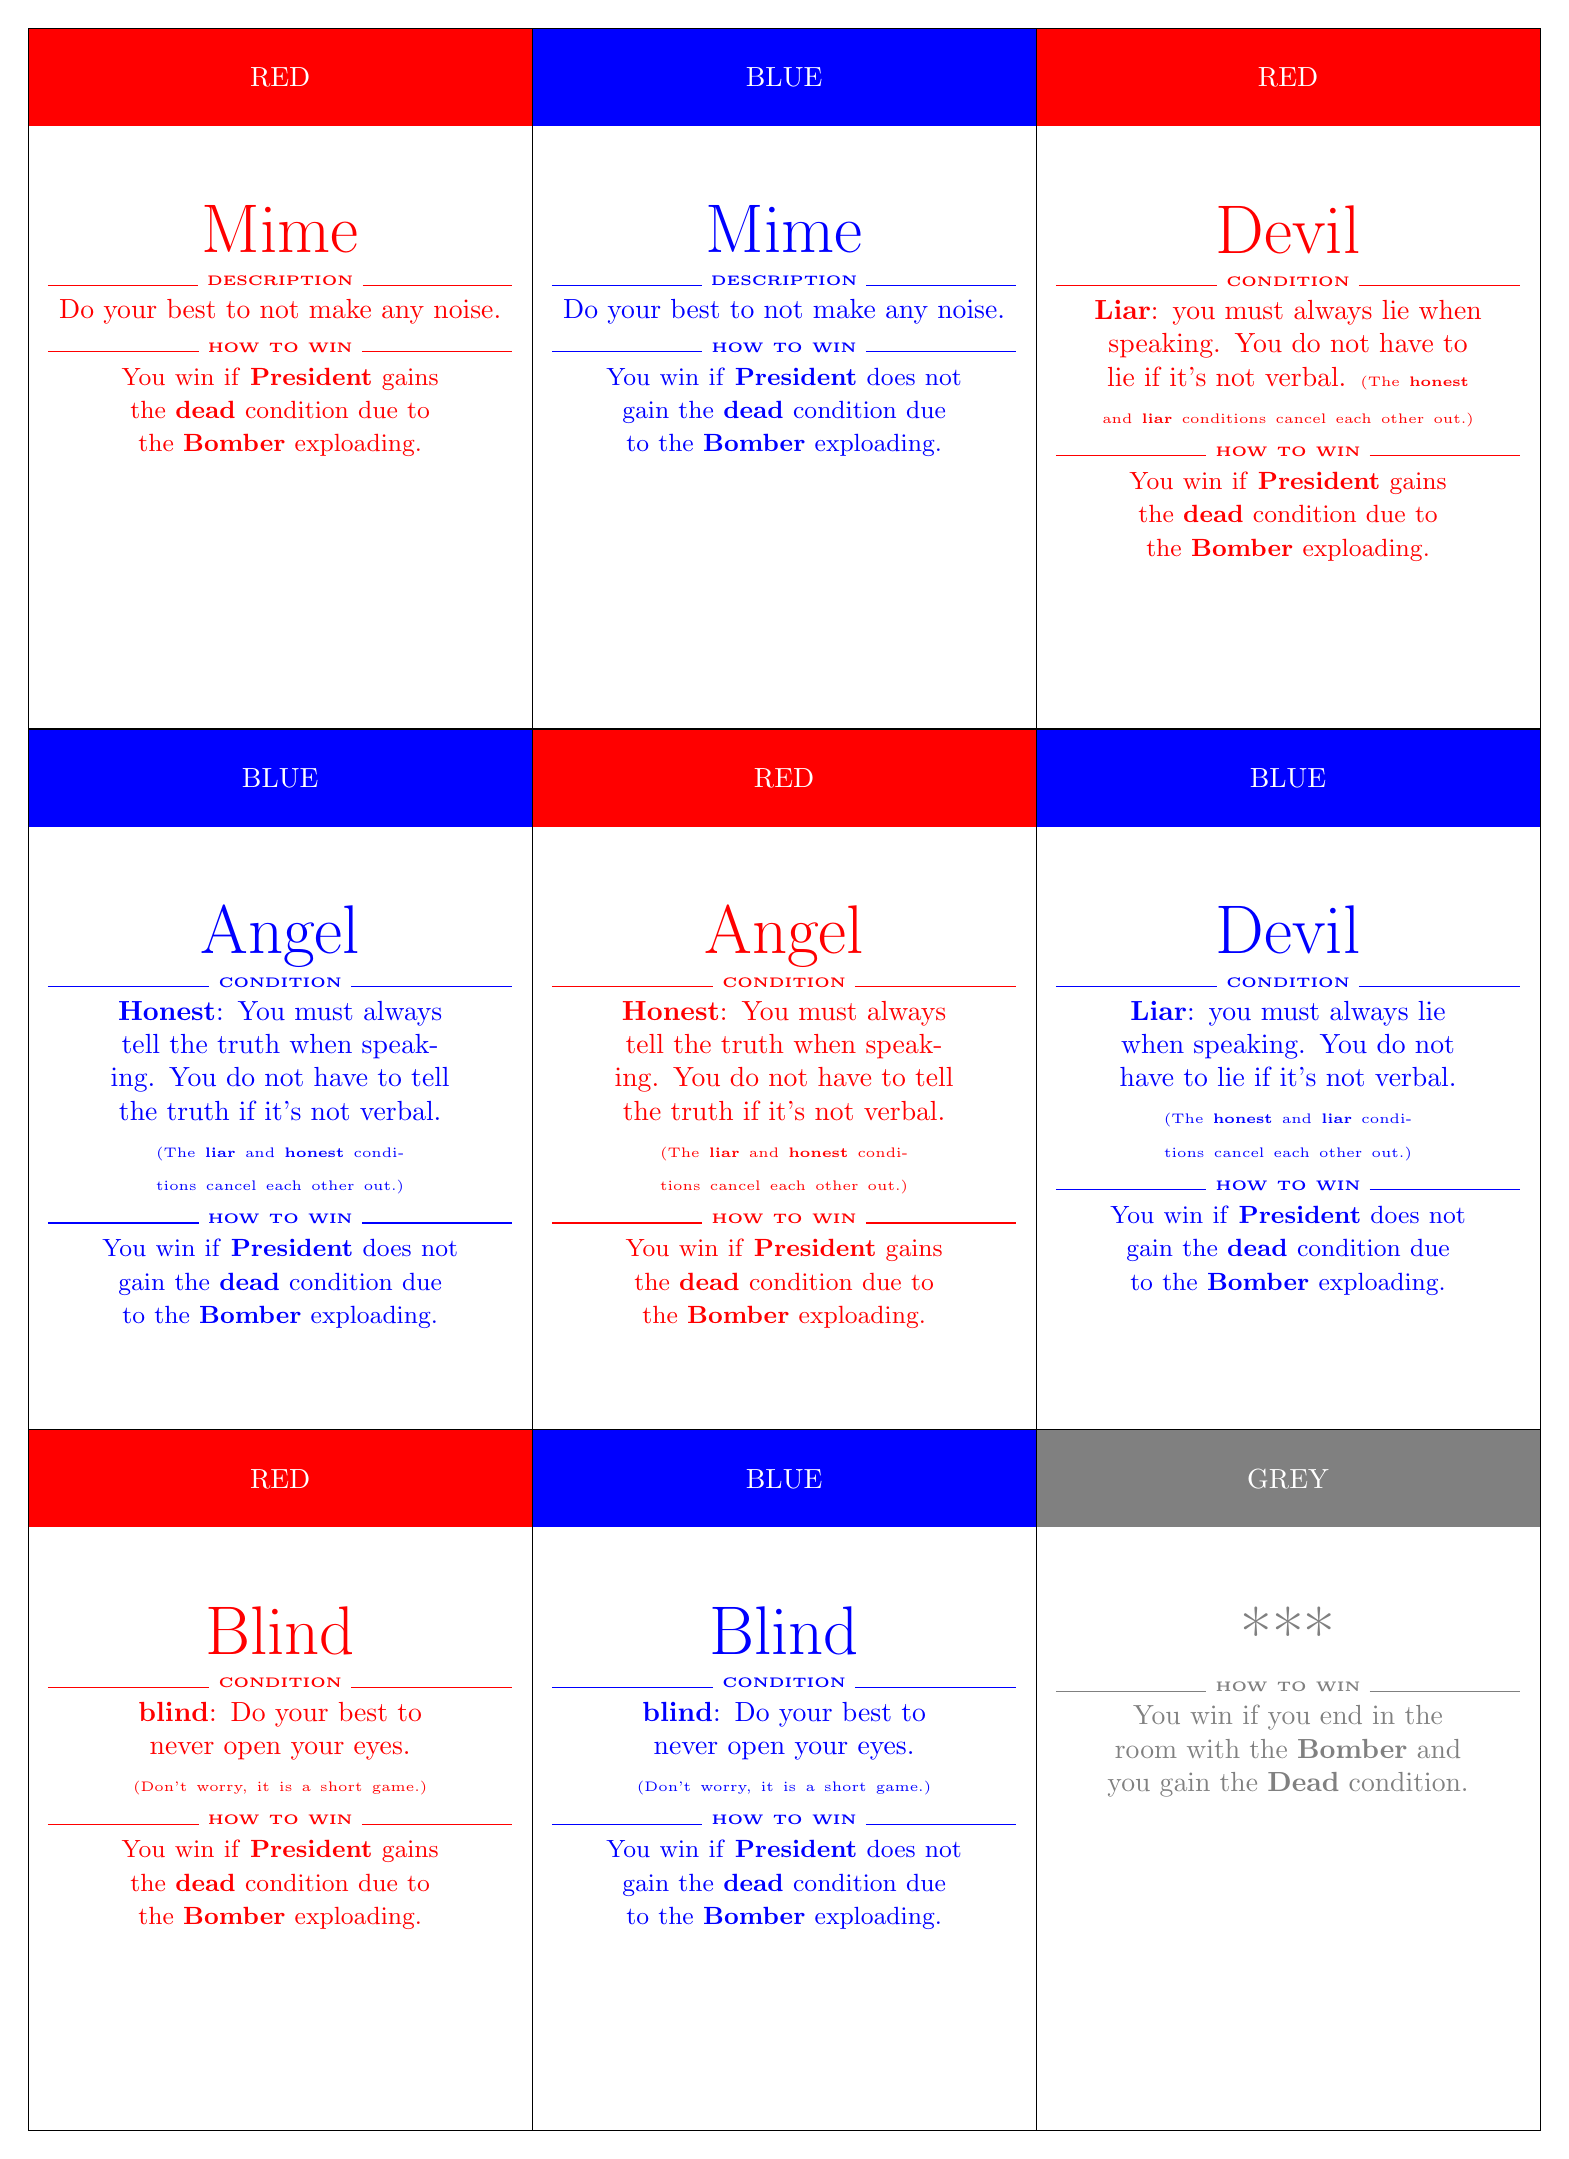
\begin{tikzpicture}[outer sep=0]


% MIME (RED TEAM)
\node[teamshare, fill=red] (1) at (3.2,26.7) {\HUGE RED};
\node[cardtext, text=red] at (3.2,24.7) {
	{\Huge Mime}
	\seperatordescription
	Do your best to not make any noise.
	\redwinsection
};

% MIME (BLUE TEAM)
\node[teamshare, fill=blue] at (9.6,26.7) {\HUGE BLUE};
\node[cardtext, text=blue] at (9.6,24.7) {
	{\Huge Mime}
	\seperatordescription
	Do your best to not make any noise.
	\bluewinsection
};

% DEVIL (RED TEAM)
\node[teamshare, fill=red] at (16,26.7) {\HUGE RED};
\node[cardtext, text=red] at (16,24.7) {
	{\Huge Devil}
	\seperatorcondition
	\condition{Liar}: you must always lie when speaking. You do not have to lie if it's not verbal.
	\vspace{0.05cm}
	\tiny (The \condition{honest} and \condition{liar} conditions cancel each other out.) \normalsize
	\redwinsection
};

% ANGEL (BLUE TEAM)
\node[teamshare, fill=blue] at (3.2,17.8) {\HUGE BLUE};
\node[cardtext, text=blue] at (3.2,15.8) {
	{\Huge Angel}
	\seperatorcondition
	\condition{Honest}: You must always tell the truth when speaking. You do not have to tell the truth if it's not verbal.
	\\\vspace{0.05cm}
	\tiny (The \condition{liar} and \condition{honest} conditions cancel each other out.) \normalsize
	\bluewinsection
};

% ANGEL (RED TEAM)
\node[teamshare, fill=red] at (9.6,17.8) {\HUGE RED};
\node[cardtext, text=red] at (9.6,15.8) {
	{\Huge Angel}
	\seperatorcondition
	\condition{Honest}: You must always tell the truth when speaking. You do not have to tell the truth if it's not verbal.
	\\\vspace{0.05cm}
	\tiny (The \condition{liar} and \condition{honest} conditions cancel each other out.) \normalsize
	\redwinsection
};

% DEVIL (BLUE TEAM)
\node[teamshare, fill=blue] at (16,17.8) {\HUGE BLUE};
\node[cardtext, text=blue] at (16,15.8) {
	{\Huge Devil}
	\seperatorcondition
	\condition{Liar}: you must always lie when speaking. You do not have to lie if it's not verbal.
	\\\vspace{0.05cm}
	\tiny (The \condition{honest} and \condition{liar} conditions cancel each other out.) \normalsize
	\bluewinsection
};

% BLIND (RED TEAM)
\node[teamshare, fill=red] at (3.2,8.9) {\HUGE RED};
\node[cardtext, text=red] at (3.2,6.9) {
	{\Huge Blind}
	\seperatorcondition
	\condition{blind}: Do your best to never open your eyes.
	\\\vspace{0.05cm}
	\tiny (Don’t worry, it is a short game.) \normalsize
	\redwinsection
};

% BLIND (BLUE TEAM)
\node[teamshare, fill=blue] at (9.6,8.9) {\HUGE BLUE};
\node[cardtext, text=blue] at (9.6,6.9) {
	{\Huge Blind}
	\seperatorcondition
	\condition{blind}: Do your best to never open your eyes.
	\\\vspace{0.05cm}
	\tiny (Don’t worry, it is a short game.) \normalsize
	\bluewinsection
};

% *******
\node[teamshare, fill=gray] at (16,8.9) {\HUGE GREY};
\node[cardtext, text=gray] at (16,6.9) {
	{\Huge ***}
	\seperatorwin
	You win if you end in the room with the \condition{Bomber} and you gain the \condition{Dead} condition.
};

\draw (0,0) -- (19.2,0);
\draw (0,8.9) -- (19.2,8.9);
\draw (0,17.8) -- (19.2,17.8);
\draw (0,26.7) -- (19.2,26.7);

\draw (0,0) -- (0,26.7);
\draw (6.4,0) -- (6.4,26.7);
\draw (12.8,0) -- (12.8,26.7);
\draw (19.2,0) -- (19.2,26.7);



\end{tikzpicture}

%Background is not my own. But courtesy of a user on BGG

\includepdf[pages={1}, angle=90]{cardsbackground.pdf}



\noindent 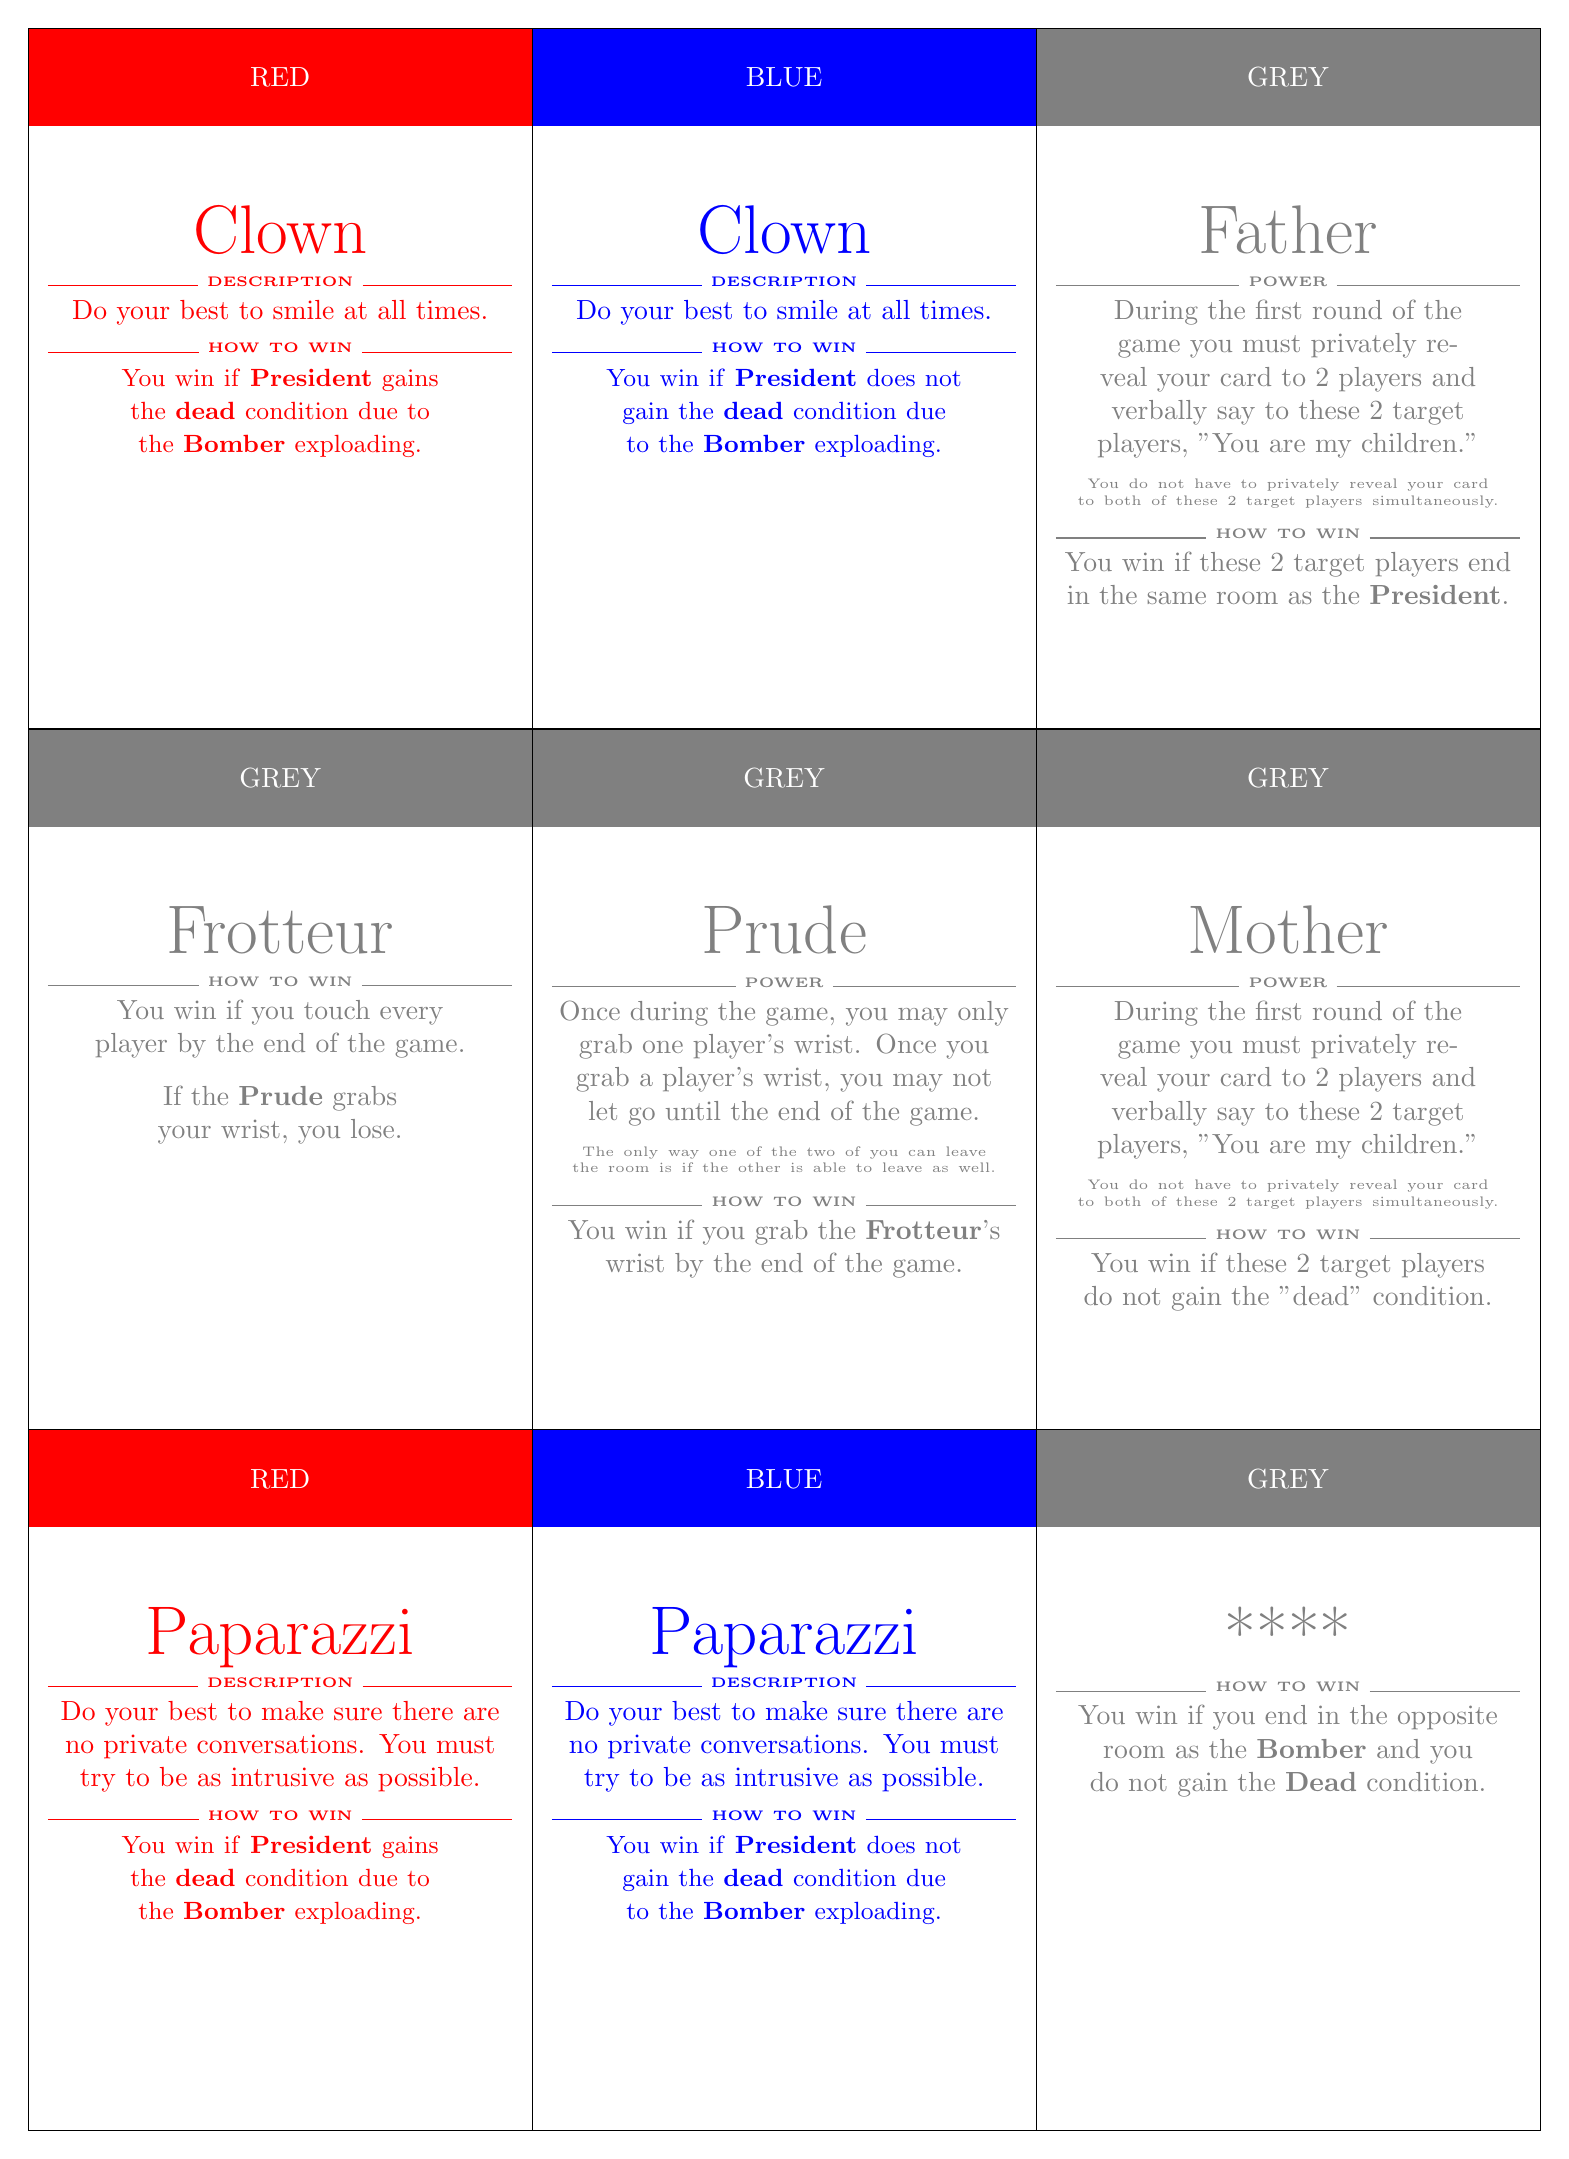
\begin{tikzpicture}[outer sep=0]

% CLOWN (RED TEAM)
\node[teamshare, fill=red] (1) at (3.2,26.7) {\HUGE RED};
\node[cardtext, text=red] at (3.2,24.7) {
	{\Huge Clown}
	\seperatordescription
	Do your best to smile at all times.
	\redwinsection
};

% CLOWN (BLUE TEAM)
\node[teamshare, fill=blue] at (9.6,26.7) {\HUGE BLUE};
\node[cardtext, text=blue] at (9.6,24.7) {
	{\Huge Clown}
	\seperatordescription
	Do your best to smile at all times.
	\bluewinsection
};

% FATHER
\node[teamshare, fill=gray] at (16,26.7) {\HUGE GREY};
\node[cardtext, text=gray] at (16,24.7) {
	{\Huge Father}
	\seperatoraction
	During the first round of the game you must privately reveal your card to 2 players and verbally say to these 2 target players, "You are my children.”
	\\\vspace{0.25cm}
	\tiny You do not have to privately reveal your card to both of these 2 target players simultaneously.
	\seperatorwin
	You win if these 2 target players end in the same room as the \character{President}.
};

% FROTTEUR (BLUE TEAM)
\node[teamshare, fill=gray] at (3.2,17.8) {\HUGE GREY};
\node[cardtext, text=gray] at (3.2,15.8) {
	{\Huge Frotteur}
	\seperatorwin
	You win if you touch every player by the end of the game.
	\\\vspace{0.25cm}
	If the \condition{Prude} grabs your wrist, you lose.
};

% PRUDE (RED TEAM)
\node[teamshare, fill=gray] at (9.6,17.8) {\HUGE GREY};
\node[cardtext, text=gray] at (9.6,15.8) {
	{\Huge Prude}
	\seperatoraction
	Once during the game, you may only grab one player’s wrist. Once you grab a player’s wrist, you may not let go until the end of the game. 
	\\\vspace{0.25cm}
	\tiny The only way one of the two of you can leave the room is if the other is able to leave as well.
	\seperatorwin
	You win if you grab the \condition{Frotteur}'s wrist by the end of the game. 
};

% MOTHER
\node[teamshare, fill=gray] at (16,17.8) {\HUGE GREY};
\node[cardtext, text=gray] at (16,15.8) {
	{\Huge Mother}
	\seperatoraction
	During the first round of the game you must privately reveal your card to 2 players and verbally say to these 2 target players, "You are my children.”
	\\\vspace{0.25cm}
	\tiny You do not have to privately reveal your card to both of these 2 target players simultaneously.
	\seperatorwin
	You win if these 2 target players do not gain the "dead" condition.
};

% PAPARAZZI (RED TEAM)
\node[teamshare, fill=red] at (3.2,8.9) {\HUGE RED};
\node[cardtext, text=red] at (3.2,6.9) {
	{\Huge Paparazzi}
	\seperatordescription
	Do your best to make sure there are no private conversations. You must try to be as intrusive as possible.
	\redwinsection
};

% PAPARAZZI (BLUE TEAM)
\node[teamshare, fill=blue] at (9.6,8.9) {\HUGE BLUE};
\node[cardtext, text=blue] at (9.6,6.9) {
	{\Huge Paparazzi}
	\seperatordescription
	Do your best to make sure there are no private conversations. You must try to be as intrusive as possible.
	\bluewinsection
};

% *****
\node[teamshare, fill=gray] at (16,8.9) {\HUGE GREY};
\node[cardtext, text=gray] at (16,6.9) {
	{\Huge ****}
	\seperatorwin
	You win if you end in the opposite room as the \condition{Bomber} and you do not gain the \condition{Dead} condition.
};

\draw (0,0) -- (19.2,0);
\draw (0,8.9) -- (19.2,8.9);
\draw (0,17.8) -- (19.2,17.8);
\draw (0,26.7) -- (19.2,26.7);

\draw (0,0) -- (0,26.7);
\draw (6.4,0) -- (6.4,26.7);
\draw (12.8,0) -- (12.8,26.7);
\draw (19.2,0) -- (19.2,26.7);



\end{tikzpicture}
%Background is not my own. But courtesy of a user on BGG

\includepdf[pages={1}, angle=90]{cardsbackground.pdf}



\end{document}